\documentclass[aima203_lecturenotes_ku.tex]{subfiles}

\setcounter{chapter}{6}
\begin{document}
\chapter{Solving Ordinary Differential Equations}
\section{Introduction}
The analytical methods of solution can be applied to solve only a selected class of differential equations. Those equations which govern physical systems do not possess, in general \textbf{closed-form} solutions, and hence recourse must be made to numerical methods for solving such differential equations. To describe various numerical methods for the solution of ordinary differential equations, we consider the general first order initial value problem. The methods so developed can, in general, be applied to the solution of first order equations.\\[2mm]
\textbf{Initial Value Problem:} \hspace{3mm} The general first order initial value problem is of the form:
\begin{equation}
  \label{ivp}
y' = f(x,y), \hspace{3mm} y(x_0) = y_0
\end{equation}
In general there are two classes of the methods for solving ~\ref{ivp}.
\begin{enumerate}
\item A series solution.
  \begin{enumerate}
  \item Taylor series method
  \item Picard method
  \end{enumerate}
\item A set of tabulated values of $x$ and $y$.
  \begin{enumerate}
  \item Euler's methods
    \item Runge-Kutta methods
  \end{enumerate}
\end{enumerate}

\section{Taylor's series method}
We consider the IVP ~\ref{ivp}. If $y(x)$ is the exact solution of this IVP, then the Taylor's series for $y(x)$ around $x=x_0$ is given by
\begin{equation}
  \label{ivptay}
  y(x) = y_0 + (x-x_0)y'_0 + \frac{(x-x_0)^2}{2!}\, y''_0 + ...
\end{equation}
Differentiating ~\ref{ivp} successively, with respect to $x$, we obtain, $y'', y''', ...$. Since ~\ref{ivptay} is an infinite series, for $y(x_0)$ correct to $N$ decimal places we solve the following equation \\
$n^{th}$ term of Taylor series $\leq$ Upper limiting error  $\displaystyle \implies \frac{(x-x_0)^n}{n!} \, f^{(n)} (x_0) \leq \frac{1}{2} 10^{-N}$. \\[1mm]
If this holds then, the $n$ number of terms is sufficient otherwise, we need to include additional terms.
\begin{figure}[h]
  \centering
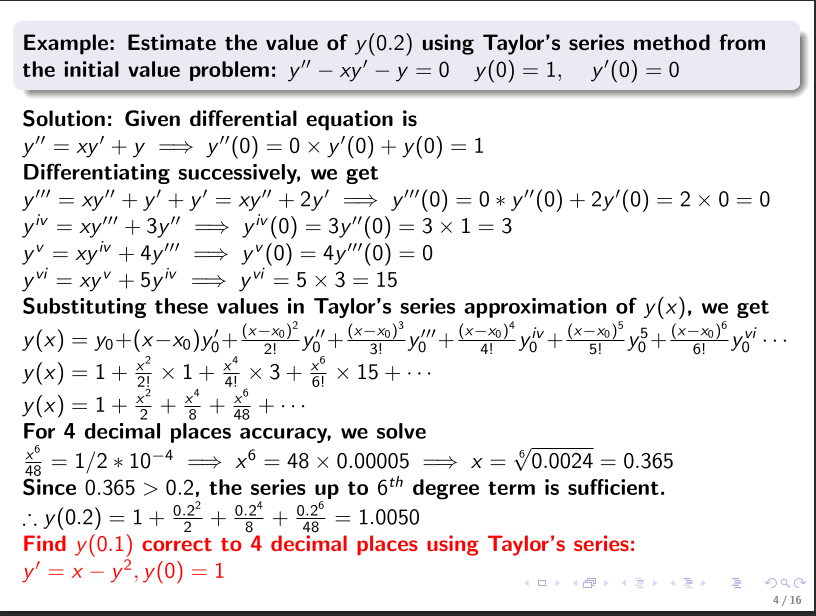
\includegraphics[width=13cm, height=10cm]{taylor_method_example.png}
\end{figure}

\section{Picard's Method of Successive Approximation}
Integrating the above differential equation ~\ref{ivp}, as follows, we obtain:
\begin{equation}
  \label{picard1}
  \begin{gathered}[b]
    \int_{x_0}^x \; y'\,dx = \int_{x_0}^x \; f(x,y)\,dx \\
      y = y_0 + \int_{x_0}^x \; f(x,y)\,dx
  \end{gathered}
\end{equation}
This equation in which the unknown function $y$ appears under the integral sign is called an \textit{integral equation}. Such equation can be solved by the method of successive approximations as follows:
\begin{equation}
  \label{picard2}
  y^{(1)} = y_0 + \int_{x_0}^x \; f(x,y_0)\,dx
\end{equation}
Proceeding in this way, we obtain:
\begin{equation}
  \label{picardit}
    y^{(n)} = y_0 + \int_{x_0}^x \; f(x,y^{(n-1)})\,dx \hspace{5mm} \text{with} \hspace{3mm}  y^{(0)} = y_0
\end{equation}
It has been proved that if $f(x,y)$ is bounded in some region about the point $(x_0, y_0)$ and if $f(x,y)$ satisfies the \textit{Lipschitz condition}, viz.,
\begin{equation*}
  |f(x,y)-f(x,\overline{y})| \leq K |y - \overline{y}|
\end{equation*}
for some constant $K$, then the sequence $y^{(n)}$ converges to the solution of the equation ~\ref{ivp}.
\begin{figure}[h]
  \centering
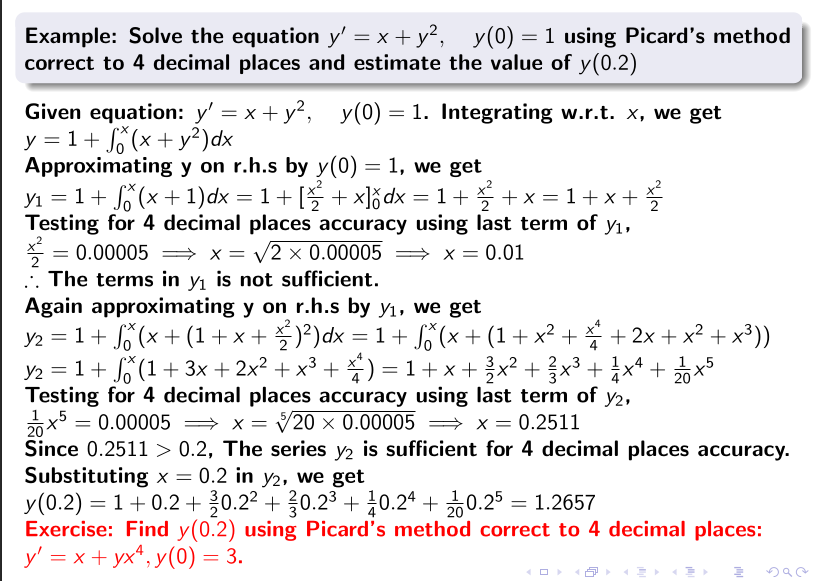
\includegraphics[width=13cm, height=10cm]{picard_method_example.png}
\end{figure}
\subsection{Exercise}
\begin{enumerate}
    \item Find by Taylor's series method:
\begin{enumerate}
    \item the value of $y(0.1)$ given that $y'=x-y^2$, $y(0)=1$.

    \item the value of $y(0)=1$ given that $\displaystyle \frac{dy}{dx} = 1 + xy$ correct up to four decimal places.
    \end{enumerate}
\item Use Picard's method to obtain:
\begin{enumerate}
    \item $y(0.1)$ and $y(0.2)$ given that $\displaystyle \frac{dy}{dx} = x + yx^4, \;\;\; y(0)=3$.
    \item $y(0.1)$ given that $\displaystyle \frac{dy}{dx} = \frac{y-x}{y+x}, \;\;\; y(0)=1$.
    \end{enumerate}
\end{enumerate}

\section{Euler's Method}
We have so far discussed the methods which yield the solution of a differential equation in the form of a power series. We will now describe the methods which give the solution in the form of a set of tabulated values. The approximation of the IVP ~\ref{ivp} by the following iteration formula is called Euler's method.
\begin{equation}
  \label{eq:9}
  y_{n+1} = y_n + h\,f(x_n,y_n) \hspace{10mm} n=0,1,2,...
\end{equation}
This formula is obtain from the forward difference $\left [ \displaystyle \frac{y_{n+1} -y_n}{h} = y'_{n} \right ]$.

\subsection{Backward Euler's Method}
Using the backward difference $\left [ \displaystyle \frac{y_{n+1} -y_n}{h} = y'_{n+1} \right ]$; we obtain, Backward Euler's Method as follows:
\begin{equation}
  \label{eq:9}
  y_{n+1} = y_n + h\,f(x_{n+1}, y_{n+1}) \hspace{10mm} n=0,1,2,...
\end{equation}
We obtain $y_{n+1}$ in $f(x_{n+1}, y_{n+1})$ from the Euler's forward method. Actually, \\
$y^{1}_{n+1} = y_n + h\,f(x_n,y_n) \hspace{5mm} n=0,1,2,...$ and $y_{n+1} = y_n + h\,f(x_{n+1}, y^{1}_{n+1}) \hspace{10mm} n=0,1,2,...$
\begin{figure}[h]
  \centering
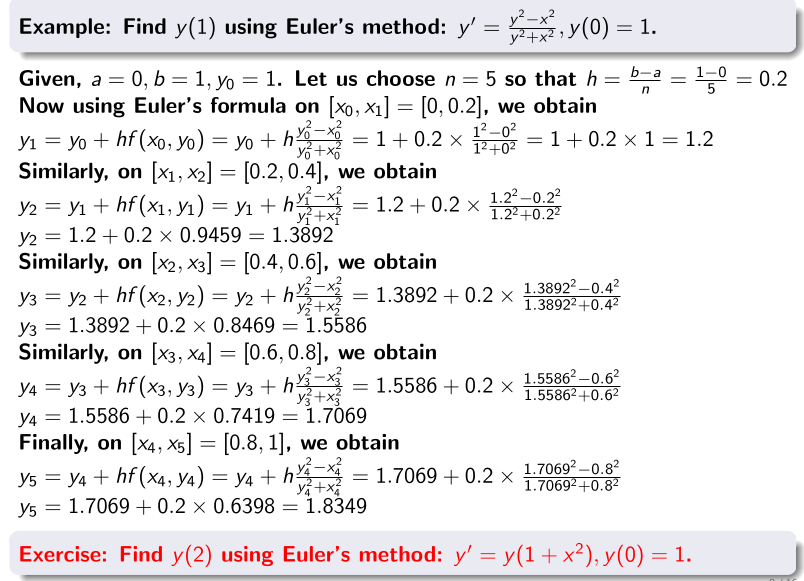
\includegraphics[width=13cm, height=10cm]{euler.png}
\end{figure}
\subsection{Modified Euler's Method}
In the Modified Euler's Method the formula for iteration is
\begin{equation}
  \label{eq:9}
  \begin{gathered}[b]
    y^{1}_{n} = y_n + h\,f(x_n,y_n) \hspace{5mm} n=0,1,2,... \\[1mm]
     y_{n+1} = y_n + \frac{h}{2} \,\left [ f(x_n,y_n) + f(x_{n+1} + y^{1}_{n}) \right ]
  \end{gathered}
\end{equation}
\subsection{Exercise}
\begin{enumerate}
    \item Use Euler's method to find $y(0.5)$ using $h=0.1$:
    \begin{multicols}{2}
        a). $\displaystyle \frac{dy}{dx}=\frac{3}{5}x^3y, \;\;\; y(0)=1$
        \columnbreak

        b). $\displaystyle \frac{dy}{dx}=1+y^2, \;\;\; y(0)=0$
    \end{multicols}

    \item Use Euler's modified method to find $y(0.2)$ and $y(0.4)$ using $h=0.2$:\\  $\displaystyle \frac{dy}{dx}=x+y, \;\;\; y(0)=0$.
    \end{enumerate}

\begin{figure}[h!]
  \centering
  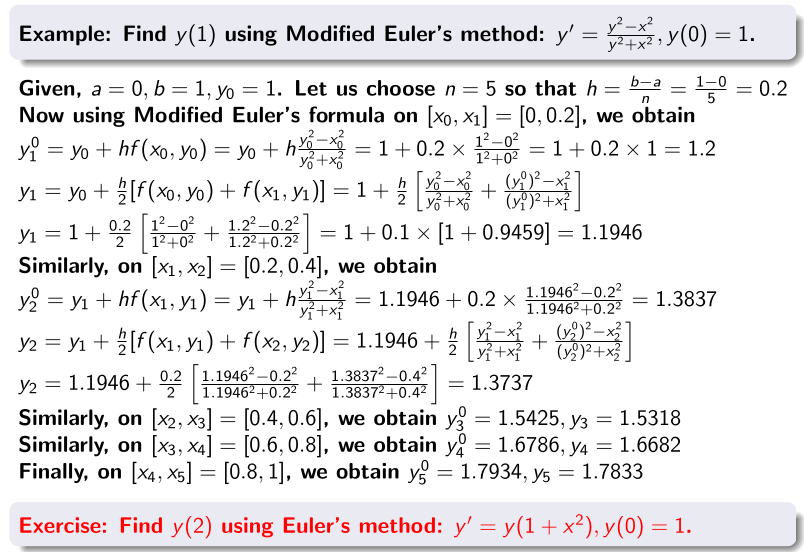
\includegraphics[width=14cm, height=10cm]{modified.png} \\[2cm]

  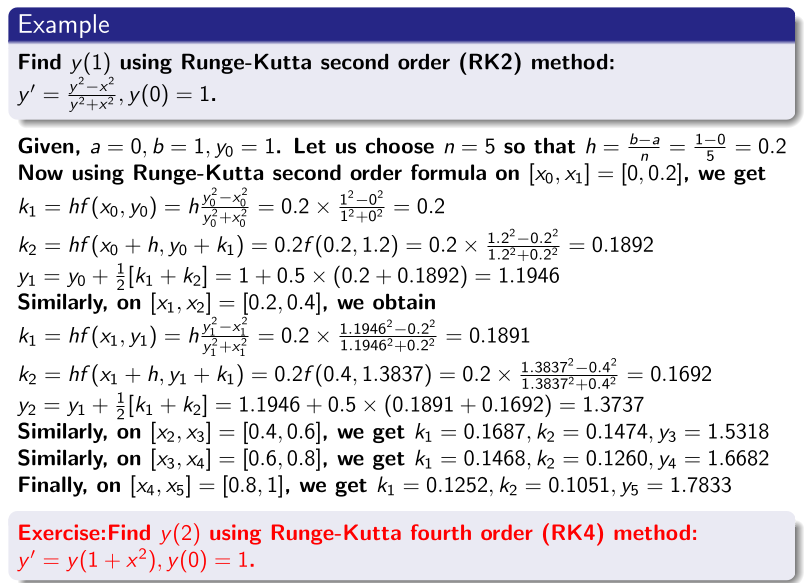
\includegraphics[width=14cm, height=10cm]{rungee.png}
\end{figure}
\section{Runge-Kutta Methods}
Euler's method is less efficient in practical problems. It requires $h$ to be small for obtaining reasonable accuracy. To overcome this issue, Runge-Kutta methods are designed.
Let $k_0 =hf(x_0,y_0)$ and $k_1 = hf(x_1, y_0 + hf(x_0,y_0)$. The special case of second order Runge-Kutta Method gives $\displaystyle y_1 = y_0 + \frac{h}{2}(k_0 + k_1)$, which is equivalent to Modified Euler's Method. So, the iteration formula for the \textbf{second-order Runge-Kutta Method} is:
\begin{equation}
  \label{rungesecond}
  \begin{aligned}[b]
    k_n &= f(x_n,y_n) \\[1mm]
    k_{n+1} &= f(x_{n+1},y_n + hk_n) \\[1mm]
    y_{n+1} &= y_n + \frac{h}{2} \,\left [ k_n + k_{n+1} \right ]
  \end{aligned}
\end{equation}

\subsection{Fourth-Order Runge-Kutta Method}
The iteration formula for the Fourth-Order Runge-Kutta method is as follows:
\begin{equation}
  \label{rungefourth}
  \begin{aligned}[b]
    k_n &= f(x_n,y_n) \\[1mm]
    k_{n+1} &= f(x_n +(h/2) ,y_n + (h/2)k_n) \\[1mm]
    k_{n+2} &= f(x_n +(h/2) ,y_n + (h/2)k_{n+1}) \\[1mm]
    k_{n+3} &= hf(x_n + h ,y_n + hk_{n+2}) \\[1mm]
    y_{n+1} &= y_n + \frac{h}{6} \,\left [k_n + 2k_{n+1} + 2k_{n+2} + k_{n+3}\right ]
  \end{aligned}
\end{equation}
\subsection{Exercise}
\begin{enumerate}
    \item Use Runge-Kutta fourth order formula
    \begin{enumerate}
        \item to find $y(0.2)$ and $y(0.4)$ given $\displaystyle y'=\frac{y^2-x^2}{y^2+x^2}, \;\;\; y(0)=1$.

        \item to find $y(1.2)$ and $y(1.4)$ given $\displaystyle y'=\frac{3x+y}{x+2y}, \;\;\; y(1)=1$.

        \item to find $y(0.2)$ given $\displaystyle y'' +y=0, \;\;\; y(0)=1, \;\; y'(0)=0$.
    \end{enumerate}

  \item Given $\displaystyle \frac{dy}{dx}=y(1+x^2), \;\;\; y(0)=1$ find the values for $x=0.2, 0.4, 0.6$ using the Euler, the modified Euler, and the fourth order Runge-Kutta methods. Compare the results thus obtained.
  \item Solve the boundary value problems by finite difference method taking $y(0)=0, \;\; y(1)=1$ for $y=0.5, 0.25$:
    \hspace{3mm} a). $y''-y=0$ \hspace{7mm} b).$y''-x^2y'-e^xy=1/(1+x)$
\end{enumerate}

\section{Simultaneous and Higher Order Equations}
Consider a pair simultaneous equations:
\begin{equation}
  \label{simul}
  \frac{dy}{dt} = f(t,x,y) \hspace{5mm} \text{and} \hspace{5mm}  \frac{dx}{dt} = g(t,x,y)
\end{equation}
with the initial conditions $x=x_0$ and $y=y_0$ when $t=t0$. Assuming that $\Delta t =h$, $\Delta x=k$, and $\Delta y = l$, the fourth order Runge-Kutta method gives,
\begin{equation}
  \label{rungesimul}
  \begin{aligned}[b]
    k_n &= f(t_n,x_n,y_n) \\[1mm]
    l_n &= g(t_n,x_n,y_n) \\[1mm]
    ... \\[2mm]
    y_{n+1} &= y_n + \frac{h}{6} \,\left [k_n + 2k_{n+1} + 2k_{n+2} + k_{n+3}\right ] \\[1mm]
    x_{n+1} &= x_n + \frac{h}{6} \,\left [l_n + 2l_{n+1} + 2l_{n+2} + l_{n+3}\right ]
  \end{aligned}
\end{equation}

We now consider the second-order differential equation:
\begin{equation}
  \label{secondorder}
  y''=F(x,y,y'), \hspace{5mm} y(x_0)=y_0, \hspace{3mm} y'(x_0) = y'_0
\end{equation}
By setting $z=y'$, the above equation ~\ref{secondorder} becomes a system of first order equations in two equations.
\begin{equation}
  \label{secondorderreduced}
  y'=z, \hspace{3mm} z'=F(x,y,z), \hspace{5mm} y(x_0)=y_0, \hspace{3mm} z(x_0) = y'_0
\end{equation}

\section{Boundary Value Problems}
The second order ordinary differential equation consists of two boundary equations as follows:
$$F(x,y,y',y'')=0, \hspace{5mm} y(x_0) = a, \hspace{3mm} y(x_{n}) = b $$
One of the popular method of solution to this boundary value problem is the method of finite difference.

\section{Finite-Difference Method}
The finite difference method for the solution of a two-point boundary value problem consists in replacing the derivatives occurring in the differential equation (and in the boundary conditions as well) by means of their finite-difference approximations and then solving the resulting linear system of equations by a standard procedure. We have the following finite difference formula for the derivatives.
\begin{enumerate}
\item \textbf{Forward Difference}
  \begin{multicols}{2}
    a). $\displaystyle y'(x) \approx \frac{y(x+h) - y(x)}{h}$

    \columnbreak
    b). $\displaystyle y''(x) \approx \frac{y(x+2h) - 2y(x+h) +y(x)}{h^2}$
  \end{multicols}

  \textbf{Backward Difference}
  \begin{multicols}{2}
    a). $\displaystyle y'(x) \approx \frac{y(x) - y(x-h)}{h}$

    \columnbreak
    b). $\displaystyle y''(x) \approx \frac{y(x) -2y(x-h) + y(x-2h)}{h^2}$
  \end{multicols}

\item \textbf{Central Difference}
  \begin{multicols}{2}
    a). $\displaystyle y'(x) \approx \frac{y(x+h) - y(x-h)}{2h}$

    \columnbreak
    b). $\displaystyle y''(x) \approx \frac{y(x+h) - 2y(x)+ y(x-h)}{h^2}$
  \end{multicols}
\end{enumerate}
These formulae can be easily derived by expanding $y(x)$ in the neighborhood of $x$ using Taylor's series. In general for higher order derivatives central difference formula gives better accuracy so,this formula is commonly used.

\subsection{General Method:}
To solve the boundary-value problem ~\ref{bvp}:
\begin{equation}
  \label{bvp}
  y'' + f(x)y' + g(x)y = r(x), \hspace{5mm} y(x_0) = a, \hspace{3mm} y(x_{n}) = b
\end{equation}

\begin{enumerate}
\item First we divide the range $[x_0, x_n]$ into $n$ equal subintervals of width $h$ so that \\ $x_i = x_0 + ih, \hspace{2mm} i=1,2,...,n$.

\item Then $y(x_i) = y_i$ and $\displaystyle y'_i = \frac{y_{i+1} - y_{i-1}}{2h}$ and $\displaystyle y''_i = \frac{y_{i+1} - 2y_i+ y_{i-1}}{h^2}$.

\item Substituting these values in ~\ref{bvp} we get,
  \begin{equation*}
    \frac{y_{i+1} - 2y_i+ y_{i-1}}{h^2} + f_i \frac{y_{i+1} - y_{i-1}}{2h} + g_i y_i = r_i, \hspace{10mm} i=1,2,...,n-1
  \end{equation*}
\item Multiplying through $2h^2$, and gathering the like terms, we get,
  $$(2-hf_i)y_{i-1} + 2(g_ih^2 -4)y_i + (2+hf_i)y_{i+1} = 2r_ih^2, \hspace{10mm} i=1,2,...,n-1 $$ with $y_0 = a, \hspace{3mm} y_n = b$.
  This comprise of a system of linear equations which can be solved with a suitable method to obtain the solution of the original differential equation ~\ref{bvp}.
 \end{enumerate}

\begin{example}
  Solve: $y'' - cosx\, y' -sinx \, y = e^x, \hspace{10mm} y(0)=0, \hspace{3mm} y(1)=1$ \\
  \textbf{Solution Steps:}
  \begin{enumerate}
  \item   Here, $x_0 = 0$ and $x_n = 1$. Choosing $n=4$ we get $h = (1-0)/4 = 0.25$.

  \item At $x=x_i$ we have $\displaystyle \frac{y_{i+1} - 2y_i+ y_{i-1}}{h^2} -cosx_i \; \frac{y_{i+1} - y_{i-1}}{2h} - sinx_i \; y_i = e^{x_i}$ \\[1mm]
    Substituting $h=0.25$, we  get, $\displaystyle \frac{y_{i+1} - 2y_i+ y_{i-1}}{(0.25)^2} -cosx_i \; \frac{y_{i+1} - y_{i-1}}{2(0.25)} - sinx_i \; y_i = e^{x_i}$

\item Simplifying: $(16+2cosx_i)y_{i-1} + (sinx_i-32)y_i + (16 -2cosx_i)y_{i+1} = e^{x_i}$


\item Substituting $x_0=0, \;\;\; x_1=0.25, \;\;\; x_2=0.5, \;\;\; x_3= 0.75$ and $y_0=1, \;\;\; y_4=1$:
  \begin{align*}
    (16+2cos(0.25))0 + (sin(0.25)-32)y_1 + (16 -2cos(0.25))y_2 &= e^{0.25} \\[1mm]
    (16+2cos(0.5))y_1 + (sin(0.5)-32)y_2 + (16 -2cos(0.5))y_3 &= e^{0.5} \\[1mm]
    (16+2cos(0.75))y_2 + (sin(0.75)-32)y_3 + (16 -2cos(0.75))1 &= e^{0.75}
  \end{align*}

\item Simplifying:
  \begin{equation}
    \label{examplesystem}
  \begin{aligned}[c]
    -32.24\, y_1 + 14.06 \, y_2 &= 1.28 \\[1mm]
    17.75 \, y_1 - 32.48\, y_2 14.24 \, y_3 &= 1.64 \\[1mm]
    17.46 \, y_2  -32.68\, y_3 + 14.54 &= 2.11
  \end{aligned}
\end{equation}

\item Solving: $y_1 = 0.01, \;\;\; y_2=0.38, \;\;\; y_3=0.98$.
  \end{enumerate}

\end{example}
\end{document}

%%% Local Variables:
%%% mode: LaTeX
%%% TeX-master: t
%%% End:
